% Options for packages loaded elsewhere
\PassOptionsToPackage{unicode}{hyperref}
\PassOptionsToPackage{hyphens}{url}
%
\documentclass[
]{article}
\usepackage{amsmath,amssymb}
\usepackage{iftex}
\ifPDFTeX
  \usepackage[T1]{fontenc}
  \usepackage[utf8]{inputenc}
  \usepackage{textcomp} % provide euro and other symbols
\else % if luatex or xetex
  \usepackage{unicode-math} % this also loads fontspec
  \defaultfontfeatures{Scale=MatchLowercase}
  \defaultfontfeatures[\rmfamily]{Ligatures=TeX,Scale=1}
\fi
\usepackage{lmodern}
\ifPDFTeX\else
  % xetex/luatex font selection
\fi
% Use upquote if available, for straight quotes in verbatim environments
\IfFileExists{upquote.sty}{\usepackage{upquote}}{}
\IfFileExists{microtype.sty}{% use microtype if available
  \usepackage[]{microtype}
  \UseMicrotypeSet[protrusion]{basicmath} % disable protrusion for tt fonts
}{}
\makeatletter
\@ifundefined{KOMAClassName}{% if non-KOMA class
  \IfFileExists{parskip.sty}{%
    \usepackage{parskip}
  }{% else
    \setlength{\parindent}{0pt}
    \setlength{\parskip}{6pt plus 2pt minus 1pt}}
}{% if KOMA class
  \KOMAoptions{parskip=half}}
\makeatother
\usepackage{xcolor}
\usepackage[margin=1in]{geometry}
\usepackage{graphicx}
\makeatletter
\def\maxwidth{\ifdim\Gin@nat@width>\linewidth\linewidth\else\Gin@nat@width\fi}
\def\maxheight{\ifdim\Gin@nat@height>\textheight\textheight\else\Gin@nat@height\fi}
\makeatother
% Scale images if necessary, so that they will not overflow the page
% margins by default, and it is still possible to overwrite the defaults
% using explicit options in \includegraphics[width, height, ...]{}
\setkeys{Gin}{width=\maxwidth,height=\maxheight,keepaspectratio}
% Set default figure placement to htbp
\makeatletter
\def\fps@figure{htbp}
\makeatother
\setlength{\emergencystretch}{3em} % prevent overfull lines
\providecommand{\tightlist}{%
  \setlength{\itemsep}{0pt}\setlength{\parskip}{0pt}}
\setcounter{secnumdepth}{-\maxdimen} % remove section numbering
\usepackage{fancyhdr} \usepackage{graphicx}
\ifLuaTeX
  \usepackage{selnolig}  % disable illegal ligatures
\fi
\IfFileExists{bookmark.sty}{\usepackage{bookmark}}{\usepackage{hyperref}}
\IfFileExists{xurl.sty}{\usepackage{xurl}}{} % add URL line breaks if available
\urlstyle{same}
\hypersetup{
  pdftitle={Bericht Tresquintos: Chile},
  hidelinks,
  pdfcreator={LaTeX via pandoc}}

\title{Bericht Tresquintos: Chile}
\usepackage{etoolbox}
\makeatletter
\providecommand{\subtitle}[1]{% add subtitle to \maketitle
  \apptocmd{\@title}{\par {\large #1 \par}}{}{}
}
\makeatother
\subtitle{\href{https://tresquintos.cl}{tresquintos.cl/popularidad}}
\author{}
\date{\vspace{-2.5em}aktualisiert: 2024-05-22}

\begin{document}
\maketitle

\addtolength{\headheight}{1.0cm} 
\fancypagestyle{plain}{} 
\pagestyle{fancy} 
\fancyhead[L]{\includegraphics[width = 25pt]{pc.png}}
\fancyhead[R]{\includegraphics[width = 30pt]{logo.png}}
\renewcommand{\headrulewidth}{0pt}

\textbf{Zusammenfassung}: Präsident Gabriel Boric ist seit 803 Tagen im
Amt, was etwa 55\% seiner Amtszeit entspricht (2022 - 2026).
\textbf{Trends}: Die folgenden Diagramme zeigen die aktuelle Dynamik der
Popularität. Die durchgezogenen Linien (blau/rot) stellen den linearen
Trend dar, während die gestrichelte Linie (grün) den nichtlinearen Trend
(und die jeweiligen oberen und unteren Fehlermargen) darstellt. Die
Zahlen zeigen an, dass Boric eine Zustimmung von 28.7\% und eine
Ablehnung von 63.3\% hat. \textbf{Durchschnitt}: Die Zustimmung schwankt
um -0.3\% pro Monat, während die Ablehnung um 0.3\% alle 30 Tage
schwankt. \textbf{Daten}: Dieser Bericht wurde automatisch anhand der
von Tresquintos gesammelten 316-Umfragen (ab 2022-03-11) erstellt.

\begin{figure}

{\centering 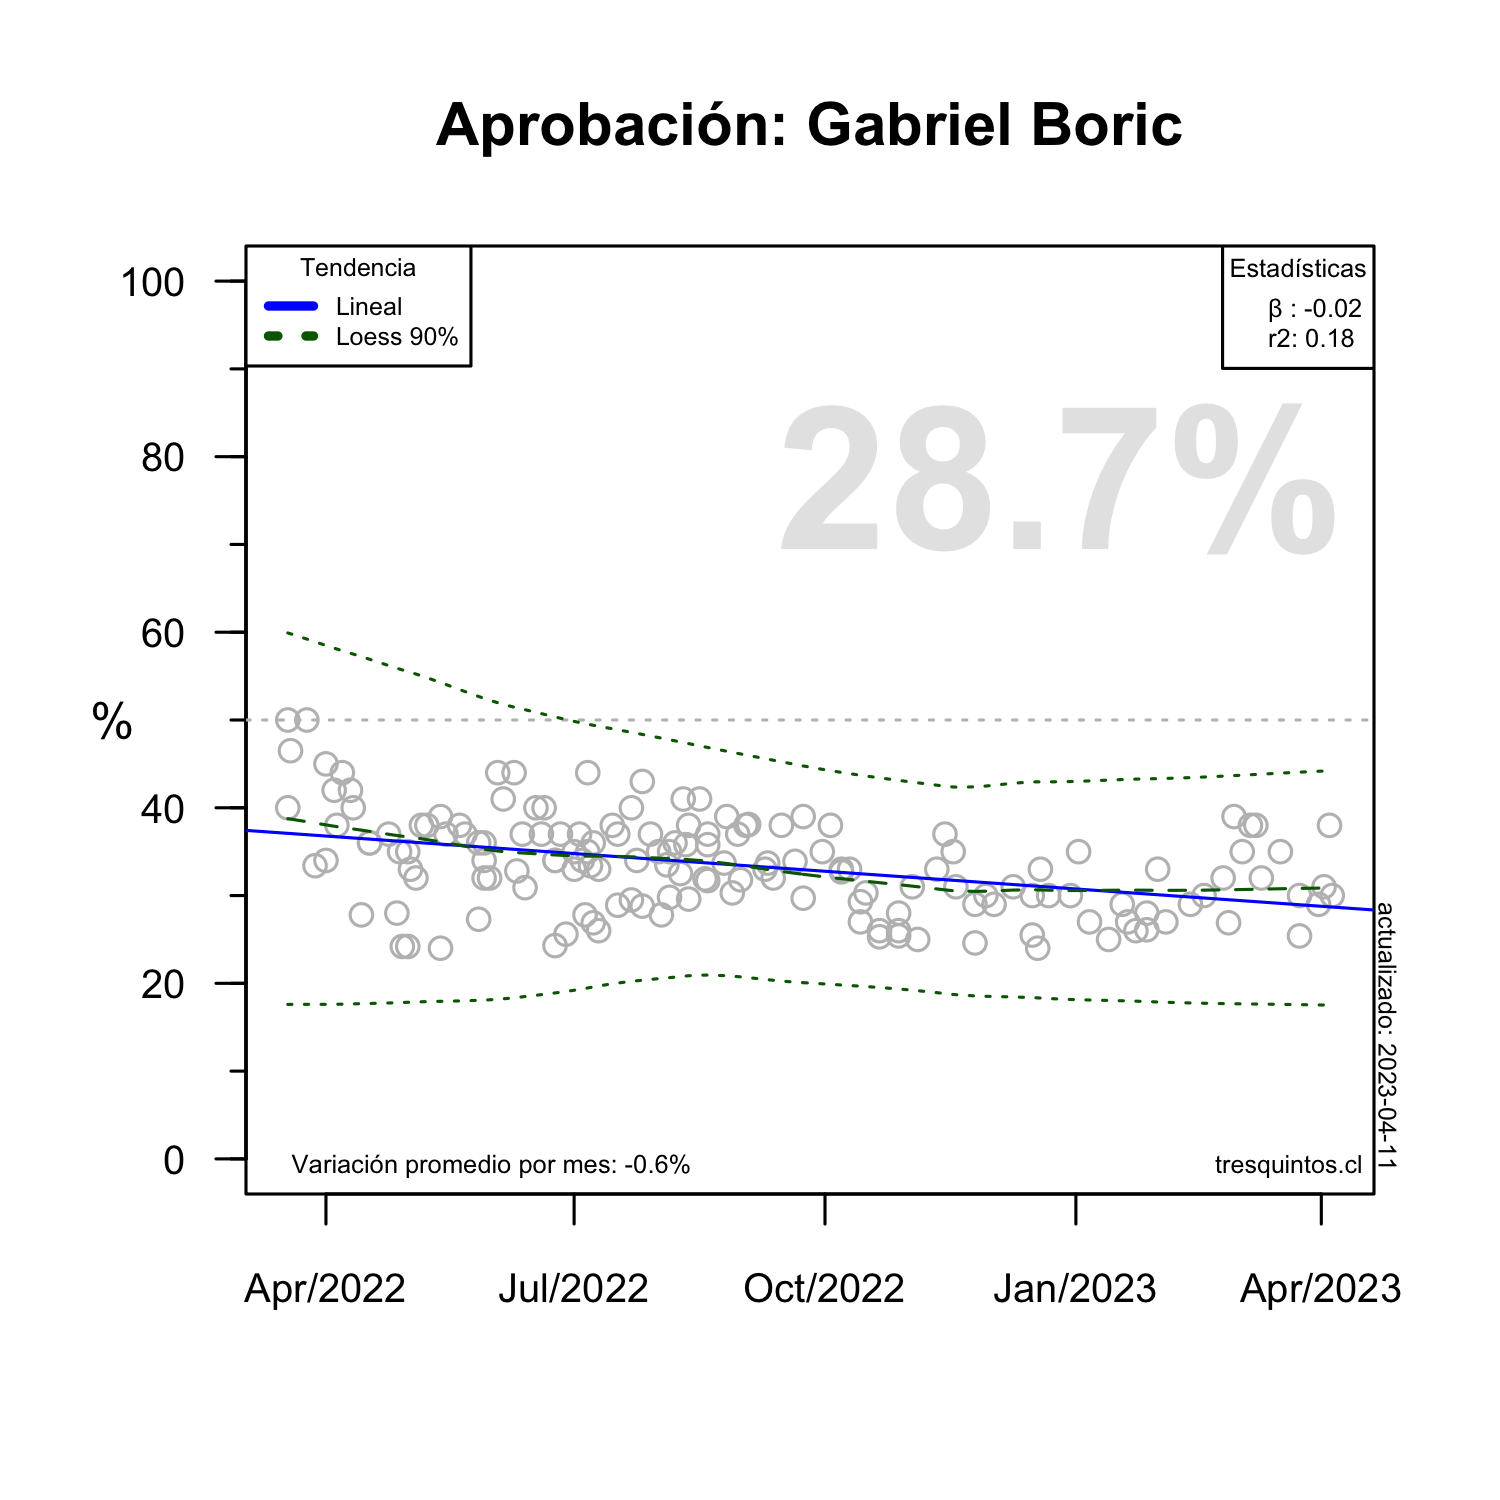
\includegraphics[width=0.49\linewidth,height=0.49\textheight]{Plots/chile-pres-aprueba} 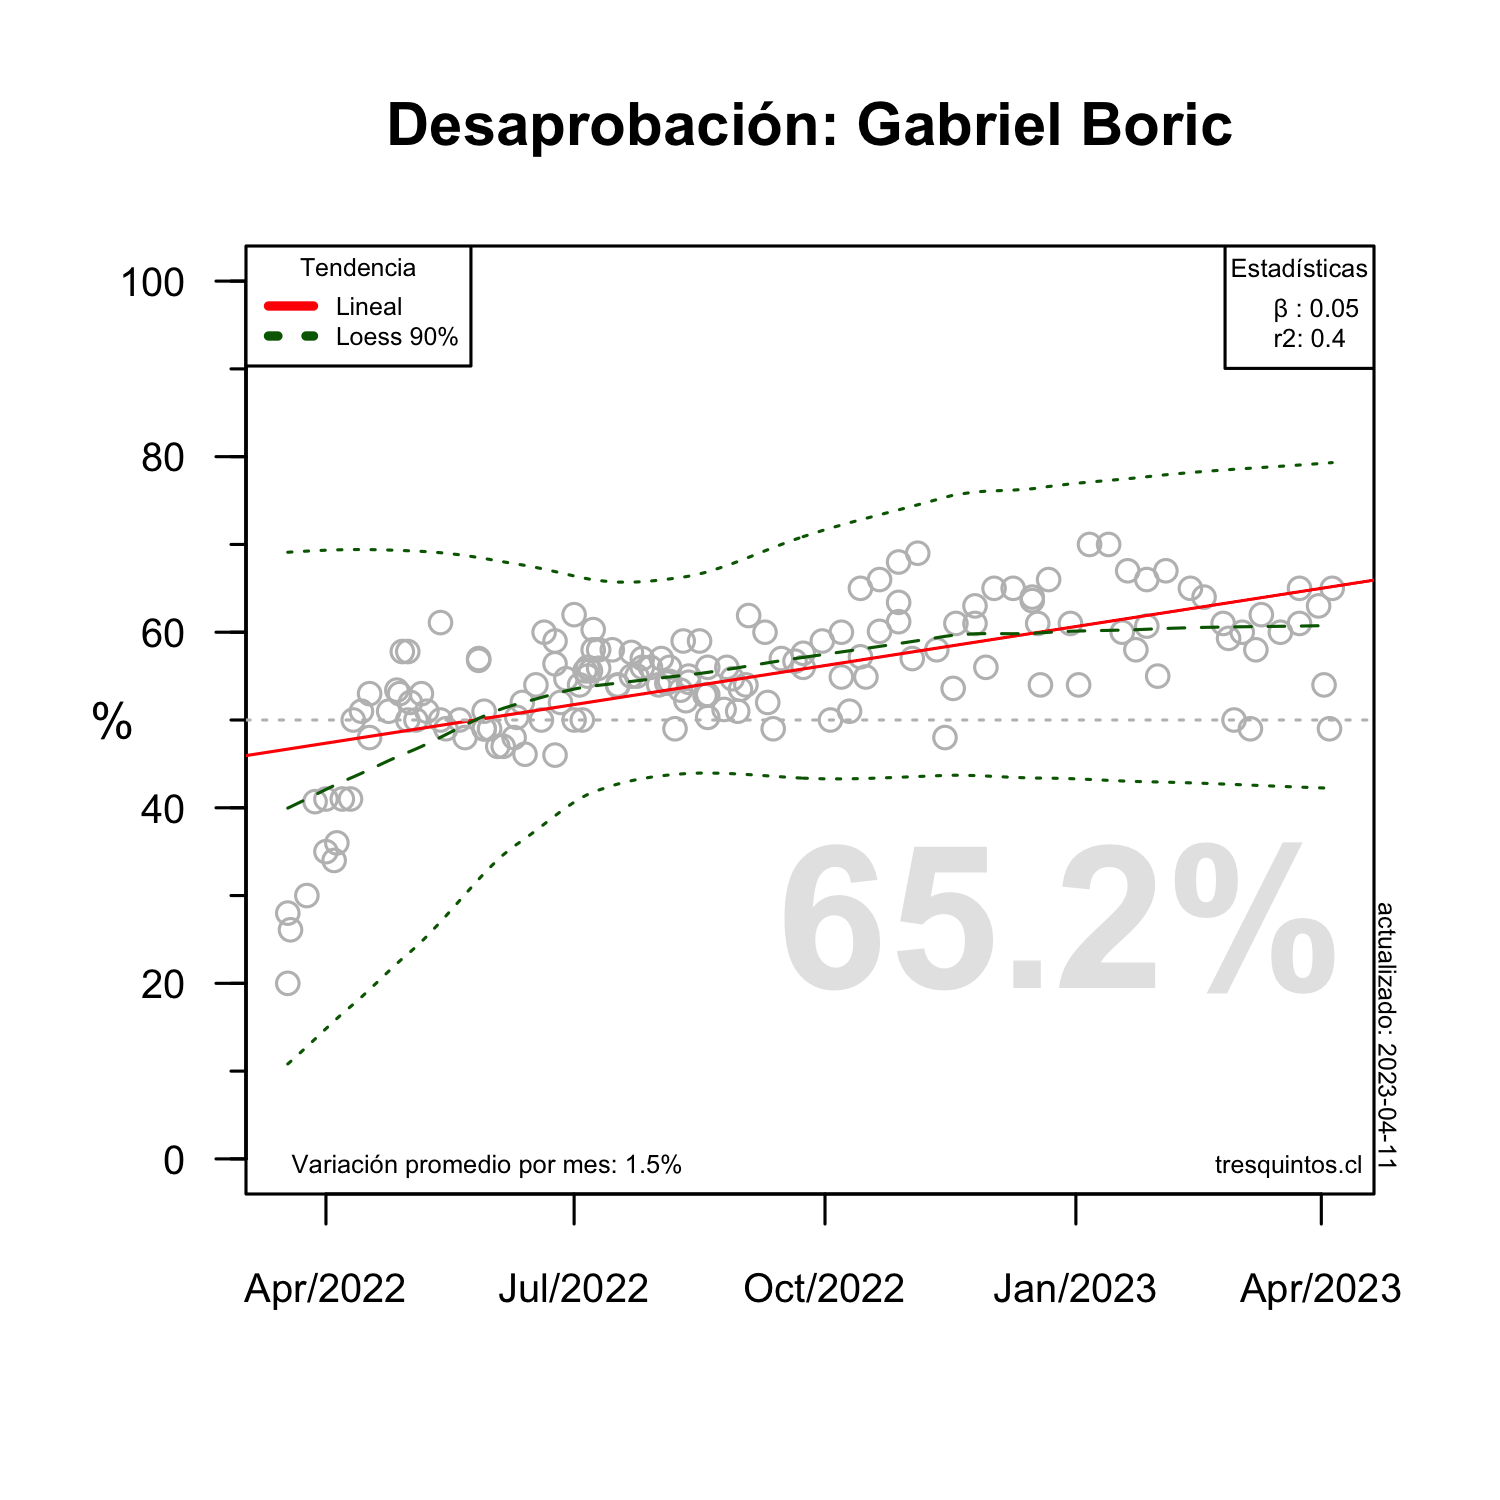
\includegraphics[width=0.49\linewidth,height=0.49\textheight]{Plots/chile-pres-desaprueba} 

}

\end{figure}

\let\thefootnote\relax

\footnote{**WARNUNG**. Dieser Bericht wird automatisch erstellt, wenn auf dem Server Unterschiede festgestellt werden. Er wird nicht von einem menschlichen Operator überwacht und kann Fehler enthalten. Für Kommentare oder Fragen, senden Sie bitte eine E-Mail an: comunicaciones@tresquintos.cl.}

\end{document}
